\documentclass[10pt]{article}

\usepackage[utf8]{inputenc}

\usepackage{amsmath,amssymb}

\usepackage{listings}

\usepackage{color}

\usepackage{graphicx}

\usepackage{float}

\usepackage{blindtext}

\usepackage{tabularx}

\usepackage{url}

\usepackage{hyperref}

\usepackage{listings}

\usepackage{caption}

\usepackage{subcaption}

\PassOptionsToPackage{hyphens}{url}\usepackage{hyperref}
\hypersetup{
	colorlinks=true,
	linkcolor=blue,
	filecolor=magenta,      
	urlcolor=cyan,
}


\usepackage{listings}
\usepackage{xcolor}

\definecolor{codegreen}{rgb}{0,0.6,0}
\definecolor{codegray}{rgb}{0.5,0.5,0.5}
\definecolor{codepurple}{rgb}{0.58,0,0.82}
\definecolor{backcolour}{rgb}{0.97,0.97,0.97}

%define Javascript language
\lstdefinelanguage{JavaScript}{
keywords={typeof, new, true, false, catch, function, return, null, catch, switch, var, if, in, while, do, else, case, break, setState, then, const},
keywordstyle=\color{codepurple}\bfseries,
ndkeywords={class, export, boolean, throw, implements, import, this, let, await},
ndkeywordstyle=\color{blue}\bfseries,
identifierstyle=\color{black},
sensitive=false,
comment=[l]{//},
morecomment=[s]{/*}{*/},
commentstyle=\color{codegreen}\ttfamily,
stringstyle=\color{red}\ttfamily,
morestring=[b]',
morestring=[b]"
}

\lstdefinestyle{mystyle}{
    backgroundcolor=\color{backcolour},   
    commentstyle=\color{codegreen},
    keywordstyle=\color{magenta},
    numberstyle=\tiny\color{codegray},
    stringstyle=\color{codepurple},
    basicstyle=\ttfamily\footnotesize,
    breakatwhitespace=false,         
    breaklines=true,                 
    captionpos=b,                    
    keepspaces=true,                 
    numbers=left,                    
    numbersep=5pt,                  
    showspaces=false,                
    showstringspaces=false,
    showtabs=false,                  
    tabsize=2
}

\lstset{style=mystyle}


\title{Design and Implementation of Mobile Applications\\plants}

\date{2020-2021}



\begin{document}
	\begin{titlepage}
		\begin{figure}[t]
			\centering
\includegraphics[width=0.7\textwidth]{resources/logo_polimi}
		\end{figure}
		\maketitle
		
		\large
		\begin{tabularx}{\linewidth}{@{}lXl@{}}
			\textit{Authors:}  & & \textit{Professors:} \\
			Federico Ferri  & & Prof.\@ Luciano Baresi\\
			Alessio Galluccio  & & Giovanni Quattrocchi\\
		\end{tabularx}		
		\thispagestyle{empty}
	\end{titlepage}
	
	\tableofcontents
	\newpage
	
	\section{Introduction}
	This document is to describe the design and the implementation of the \textit{plants} mobile application with emphasis on the user experience and the technology stack used. \\\\
	This project is the evaluation work for the Design and Implementation of Mobile Applications class at Politecnico di Milano taught by Professor Luciano Baresi and Giovanni Quattrocchi as teaching assistant.
	
	\subsection{Idea}
	The idea came from a very simple need that arose during this 2020 pandemic as many people were forced to shelter at home and thus had much more time to dedicate to hobbies and personal activities. \\\\
	During this idea generation step we both shared a common hobby which is maintaining a small home vegetable garden. \\\\
	While sharing this hobby we both shared also the same problem related to such an hobby which is watering. Watering requires a small attention span but at a very constant interval because even a single miss could cause the plants to die. \\\\
	We thus had the idea to create a specialized digital tool to manage watering but not of a single plant but of an entire garden because each plant requires different amount of water depending on many different factors.
	
	\newpage
	\subsection{Requirements}
	After coming up with the idea we started devising the functionalities of the app. The app main goal is to remind you exactly at the right time to water the plant(s) that need to be watered. \\\\
	This has to be very precise because a wrong timing on when to water the plants can damage them or make the application useless by giving too many wrong indications to the user. \\\\
	Moreover the application should keep the data and the service going regardless if a user changes phone and it must be simple to set up.\\\\
	In the end we decided to divide the requirements into functional and non functional requirements, the first being related to the core functionalities and the latters being related to a good user experience.
	
	\subsubsection{Functional requirements}
	The functional requirements are all the elements that must be present in the app to make the core requirements possible.
	\begin{itemize}
		\item Sign-in using social accounts such as Google or Facebook to ensure a fast and seamless sign-up and login experience.
		\item View in a glance your plants and their current status.
		\item Adjust the status of a plant if the application is currently wrong about it.
		\item Inform the application about relevant events for a plant such as when it has been watered.
		\item Add new plants to the application.
		\item Inform with a push notification when its time to water a plant.
		\item Use as many information as possible from the user and from external services such as the weather service to predict best when a plant needs water.
		\item Delete a plant from the application.
		\item Modify a plant from the application.
	\end{itemize}
	
	\newpage
	\subsubsection{Non functional requirements}
	The non functional requirements are as important the functional ones but related to the aspects of the application that are not core but still necessary to make the user experience enjoyable.
	\begin{itemize}
		\item The application should run both on Android and iOS with the same level of service and features.
		\item The notifications about important events should be generated and delivered in a timely manner even if the app is in deep sleep mode or frozen. 
		\item The application can use the photo camera when needed.
		\item The application can use the positioning services when needed.
		\item The user can disable push notifications if deemed too invasive.
	\end{itemize}

	\subsection{Assumptions}
	We assume to simplify the design and the development some characteristics about the environment and the device where \textit{plants} runs on.
	
	\begin{itemize}
		\item The connection to the internet is always available, reliable and with a good speed.
		\item The third parties API (application programming interface) and services are always available.
		\item The device where \textit{plants} runs on is free of any limitations that would impact the functioning of the application such as unavailable storage or too strict permission limitations.
	\end{itemize}
	
	\newpage
	\section{Design}
	\subsection{Framework}
	Our framework choice between the ones proposed in class (Flutter, React Native, Android, iOS, Progressive Web Apps) has been decided based mainly on cross platform compatibility. \\\\ The requirement already excludes pure Android and iOS development from the spectrum. \\\\We decided to land on React Native because we were inspired by the huge ecosystem of packages offered for React Native and the immense popularity it has. \\\\ We decided to exclude Flutter because it is based on DART a language that we have never used before. Moreover also Progressive Web Apps were a very interesting candidate but we felt that using them was not in the theme of the course because they are primarily developed using web technologies and adapted to be used as mobile applications.
	
	\subsection{Architecture}
	We decided to use as many external services as possible to keep the application codebase lean and to reduce the development effort. \\\\
	The system architecture consists in the \textbf{client}, the firebase services such as \textbf{Firebase authentication}, \textbf{Firestore} and \textbf{Firebase storage}. The \textbf{notification service} and the \textbf{weatherapi.com} service. Moreover we have some other services we rely upon such as the \textbf{Google authentication}, the \textbf{Facebook authentication} and the \textbf{Google cloud functions}.
	
	
	\subsubsection{Client}
	The client consists in the React Native application and is the core of the entire project. We decided to use the SDK 40 of React Native because it is a good and stable version of the SDK. \\\\ The biggest choice we made is to use Expo. Expo is a platform that allow to speed up React Native development at the expense of less freedom in terms of functionalities. We analyzed our needs and decided to proceed in using Expo due to the advantages in terms of using a real mobile device for development and being able to run it off real iOS and Android devices without having to deal with platform specific stores. \\\\ We also decided to use an approach based more on classes than function in our React Native codebase because we have often to deal with internal state of the components that compose the screen so the usage of classes is advised.
	
	For cleanliness we decided to divide the codebase into logic blocks:
	\begin{itemize}
		\item \textbf{Assets}: these represent the various binary imports of the components such as images and fonts.
		\item \textbf{Components}: the components represent some elements in a screen, we decided to group them together to reuse them as much as possible into different sections of the application.
		\item \textbf{Config}: the configuration files used to store configuration settings such as API keys.
		\item \textbf{Navigaton}: similarly as the components here we can find the elements related to navigating the various app's screens.
	\end{itemize}
	
	\subsubsection{Authentication}
	Making sure that a good authentication process is in place is not an easy task and it is often overlooked even by major mobile applications. We decided to use social sign-in to completely avoid the risks of rolling our own authentication service. \\\\ We use Firebase authentication to aggregate login data of our users and to manage authentication. As social login providers we use Google and Facebook and to enable this we registered a Facebook application to obtain a Facebook App Id and we also registered a Google application to obtain the ability to login using Google. 
	
	\subsubsection{Database and storage}
	To store all of our data we user Firestore a NoSQL database offered by Firebase. This database is quite different compared to a traditional database. It's a database that offers a client SDK to interact with. \\\\ Traditionally databases only offered interfaces for server side applications to interact with it, with Firestore it's possible to have an application that saves its state without having a custom backend. \\\\ We designed our database with these collections, collections are the equivalent of table for traditional SQL databases:
	\begin{itemize}
		\item \textbf{users}: here in each document (the equivalent of a row in a SQL database) we can find some data about user preferences in receiving notifications and its Expo notification token. The token's function will be better explained in the specific section.
		\item \textbf{plantTypes}: each document represent a specific plant type supported by the application. They are stored server side to allow adding a new plant without having to deliver a new release. Each plant type has a few characteristics parameters used by the watering algorithm.
		\item \textbf{plants}: the most important collection stores each plant added by any users and its status and history. It's a very dense collection but this is advisable in a NoSQL environment to allow for better performances since joins are not advised.
	\end{itemize}
	To store large binary files generated by users such as images we use Firebase storage a bucket service to store large files and serve them to the internet.
	
	
	\subsubsection{weatherapi.com}
	To gain information about the weather in a particular location we use a third party service. We landed on this service because it offers a nice API and moreover it serves icon to represent the weather in a graphical way.
	
	\subsubsection{Notification service}
	Notifications to the clients are not generated on the client itself in background but are generated and sent remotely. This is because many devices tend to kill or send to deep sleep and application that is not used very often to save on RAM and CPU usage. Such a behaviour would make our service useless due to unreliability. \\\\ We then decided to develop a Google cloud function that runs periodically and checks the Firestore database for upcoming events. If such events are found notifications are sent to the clients using Expo notifications. This is fine for an unpublished application in a public application available on the stores it would be wiser to use a service such as Firebase notifications.\\\\ Moreover inside Firestore as mentioned before is stored the Expo token needed to send such notifications to the device and this token is retrieved and updated on Firestore every time the user opens up the client application.
	
	\section{External Services and Libraries}
	\textit{Plants} uses a set of external services and libraries to carry out its objectives. Here we present in detail the services used.
	
	\subsection{Firebase}
	\textit{Plants} uses Firebase services to handle the server and the authentication of the user. Here we show one example of code using the Firebase package. This is the code used on refresh of the HomeScreen to retrieve the updated data of the plants.
	\begin{lstlisting}[language=JavaScript]
    onRefresh() {
    this.setState({isFetching: true});
    firebase.firestore().collection('plants').where('uid', '==', this.state.user.uid).get().then(snapshot => {
      const tmpPlants = [];
      snapshot.forEach(doc => {
        tmpPlants.push(doc);
      });
      this.setState({plants: tmpPlants, isFetching: false});
    }).catch(err => {
      console.log('Error getting documents', err);
    });
    }
	\end{lstlisting}
	\subsection{weatherapi}
	
	\textit{Plants} uses the third party service weatherapi to gain information about the weather in the location where the plant is positioned. In specific, we use this service in the front end to get the temperature, the weather condition (sunny, rainy, etc) and a icon that represents it. All this data is used in the Detail page of the plant. 
	
	In a complete implementation of the app, the weatherapi services would be used in the backend to calculate the next weathering time of each plant, since the temperature and the weather influence the needs of a plant.
	
	\begin{lstlisting}[language=JavaScript]
    //weatherapi request
    fetch('http://api.weatherapi.com/v1/current.json?key=_KEY_&q='
    +plantLatidute +','+ plantLongitude + '&aqi=no')
    .then(response => response.json())
    .then(responseJson => {
        this.setState(
        {
            icon: responseJson.current.condition.icon,
            condition_weather: responseJson.current.condition.text,
            temperature: responseJson.current.temp_c
        },
        ...
        );
	\end{lstlisting}
	
	\subsection{ImagePicker}
	The app uses the 'expo-image-picker' package to handle the process of taking the photo of the plant. This library permits the user to cut the image after taking it in order to fit the required dimensions.
	
	\begin{lstlisting}[language=JavaScript]
    //launch the camera
    let pickerResult = await ImagePicker.launchCameraAsync({
        allowsEditing: true,
        aspect: [350, 250],
        quality: 1,
      } );
    if (pickerResult.cancelled === true) {
        ...
    }
    this.setState({ plantImage: pickerResult.uri });
	\end{lstlisting}
	
	\subsection{Location}
	During the process of adding a new plant, the user is required to add the location of the plant in order to let the app use the data of the weather. 'expo-location' package is used both to handle the geolocalization and the validation of an address inserted by the user.
	
	The geolocalization retrieves the last position registered by the phone. This method permits to have a fast and accurate geolocalization, instead of starting to localize the phone when the icon of geolocalization is pressed, which was found to be too slow for the user experience.
	\begin{lstlisting}[language=JavaScript]
    //get permission to access map services
    let permission = await Location.requestPermissionsAsync();
    if (permission === false) {
        alert("Permission to access map services is required!");
        return;
    }
    //use last known position of the phone
    let location = await Location.getLastKnownPositionAsync({});
    ...
	\end{lstlisting}
	
	The validation of the address added manually by the user is done by using the method 'geocodeAsync', which provides a set of most probable coordinates in descending order, given the name of the location. The app selects the most probable one and shows it to the user, who will decide if the location found is the correct one.
	\begin{lstlisting}[language=JavaScript]
    //retrieve most probable positions, given the address inserted
    let resultLocation = await Location.geocodeAsync(textOfUser);
    //select coordinates of the most probable location
    this.setState({ latitude: resultLocation[0].latitude });
    this.setState({ longitude: resultLocation[0].longitude });
    \end{lstlisting}
	
	\newpage
	\section{Use Cases}
	In this section the different ways in which the user can interact with \textit{Plants} are showed. The focus is on the most significant interaction and on the front-end of the application.
    
    \subsection{Sign up with google account}
    \begin{tabular}{ p{3cm}|p{8cm} }
     &\textbf{Sign up with google account} \\
     \\
     Precondition & The user has a google account \\
     \\
     User flow 
     & 1. The user downloads and installs the app\\ 
     & 2. The user opens the app and is directed to the sing up/login page \\
     & 3. The user clicks the google button\\ 
     & 4. The app opens the google services on the browser to convalidate the account  \\
     & 5. The user log in with their google account\\
     & 6. The app receives the data and register it in Firebase\\
     & 7. The app redirects the user to the home page\\
     \\
     Postconditions & the user is registered to the app and they are on the homepage \\ 
     \\
     Exceptions & Data inserted by the user is not correct and the flows goes to point 3\\
    \end{tabular}
    \newline
    \newline
    \newline
    \subsection{Sign up with facebook account}
    \begin{tabular}{ p{3cm}|p{8cm} }
     & \textbf{Sign up with facebook account} \\
     \\
     Precondition & The user has a facebook account \\
     \\
     User flow  
     & 1. The user downloads and installs the app\\ 
     & 2. The user opens the app and is directed to the sing up/login page \\
     & 3. The user clicks the facebook button\\ 
     & 4. The app opens the facebook services on the browser to convalidate the account  \\
     & 5. The user log in with their facebook account\\
     & 6. The app receives the data and register it in Firebase\\
     & 7. The app redirects the user to the home page\\
     \\
     Postconditions & the user is registered to the app and they are on the homepage \\ 
     \\
     Exceptions & Data inserted by the user is not correct and the flows goes to point 2\\
    \end{tabular}
    \newline
    \newline
    \newline
    \subsection{Login with a google account}
    \begin{tabular}{ p{3cm}|p{8cm} }
     & \textbf{Login with a google account} \\
     \\
     Precondition & The user has already registered to the app with a google account \\ 
     \\
     User flow  
     & 1. The user opens the app and is directed to the sing up/login page \\
     & 2. The user clicks the google button\\ 
     & 3. The app opens the google services on the browser to convalidate the account  \\
     & 4. The user log in with their google account\\
     & 5. The app redirects the user to the home page\\
     \\
     Postconditions & The app shows the homepage to the user \\ 
     \\
     Exceptions & Data inserted by the user is not correct and the flows goes to point 1\\
    \end{tabular}
    \newline
    \newline
    \newline
    \subsection{Login with a facebook account}
    \begin{tabular}{ p{3cm}|p{8cm} }
     & \textbf{Login with a facebook account} \\
     \\
     Precondition & The user has already registered to the app with a facebook account \\ 
     \\
     User flow 
     & 1. The user opens the app and is directed to the sing up/login page \\
     & 2. The user clicks the facebook button\\ 
     & 3. The app opens the facebook services on the browser to convalidate the account  \\
     & 4. The user log in with their facebook account\\
     & 5. The app redirects the user to the home page\\
     \\
     Postconditions & The app shows the homepage to the user \\
     \\
     Exceptions & Data inserted by the user is not correct and the flows goes to point 1\\
    \end{tabular}
    \newline
    \newline
    \newline
    \subsection{Adding of a new plant}
    \begin{tabular}{ p{3cm}|p{8cm} }
     & \textbf{The user adds a new plant} \\
     \\
     Precondition & The user is on the homepage and their phone has a working camera \\ 
     \\
     User flow 
     & 1. User clicks on the "+" button in the bottom bar \\
     & 2. App navigates to "add a plant" (step 1) screen\\ 
     & 3. User inserts name of the plant, type of the plant and takes a photo of the plant with the camera  \\
     & 4. User clicks the forward arrow\\
     & 5. App navigates to "position" (step 2) screen \\
     & 6. User inserts position, exposition and adds (optionally) the name of the room \\
     & 7. User clicks the forward arrow \\
     & 8. App navigates to "address" (step 3) screen \\
     & 9. User presses the geolocalization button or inserts the address of the plant position manually \\
     & 10. User clicks the forward arrow \\
     & 11. App navigates to "How is your plant now" (step 2) screen \\
     & 12. User presses the button representing the current status of the plant (good or bad) \\
     & 13. App processes and sends all the data of the new plant to firebase \\
     & 14. App updates its data from Firebase and navigates to the homescreen \\
     \\
     Postconditions & App shows the homepage to the user and a new plant with the data inserted by the user is added \\
     \\
     Exceptions 
     & 1. User presses the backward arrow. Flows goes to the previous step\\
     & 2. User clicks the forward arrow of a page, but the required data is inserted by the user. App shows an alert and doesn't go to the next step\\
    \end{tabular}
    \newline
    \newline
    \newline
    \subsection{Visualization of the details of a plant}
    \begin{tabular}{ p{3cm}|p{8cm} }
     & \textbf{Visualization of the details of a plant} \\
     \\
     Precondition & User is on the homepage and has already added the plant \\ 
     \\
     User flow 
     & 1. User clicks the image of the widget of the plant \\
     & 2. App navigates to Detail page of the plant \\ 
     \\
     Postconditions & The app shows the details of the plant \\
     \\
     Exceptions & -\\
    \end{tabular}
    \newline
    \newline
    \newline
    \subsection{"Watering" event}
    \begin{tabular}{ p{3cm}|p{8cm} }
     & \textbf{"Watering" event} \\
     \\
     Precondition & User is on the homepage and has already added the plant \\ 
     \\
     User flow 
     & 1. User clicks on the "watering" icon of the widget of the plant \\
     & 2. App sends data of the event to firebase and updates the status of the plant \\ 
     \\
     Postconditions & Plant status is affected by the "watering" event \\
     \\
     Exceptions & -\\
    \end{tabular}
    \newline
    \newline
    \newline
    \subsection{"Good plant" event}
    \begin{tabular}{ p{3cm}|p{8cm} }
     & \textbf{"Good plant" event} \\
     \\
     Precondition & User is on the homepage and has already added the plant \\ 
     \\
     User flow 
     & 1. User clicks on the "good plant" icon of the widget of the plant \\
     & 2. App sends data of the event to firebase and updates the status of the plant \\ 
     \\
     Postconditions & Plant status is affected by the "good plant" event \\
     \\
     Exceptions & -\\
    \end{tabular}
    \newline
    \newline
    \newline
    \subsection{"Bad plant" event}
    \begin{tabular}{ p{3cm}|p{8cm} }
     & \textbf{"Bad plant" event of a plant} \\
     \\
     Precondition & User is on the homepage and has already added the plant \\ 
     \\
     User flow 
     & 1. User clicks on the "bad plant" icon of the widget of the plant \\
     & 2. App sends data of the event to firebase and updates the status of the plant \\ 
     \\
     Postconditions & Plant status is affected by the "bad plant" event \\
     \\
     Exceptions & -\\
    \end{tabular}
    \newline
    \newline
    \newline
    \subsection{Navigation to homepage}
    \begin{tabular}{ p{3cm}|p{8cm} }
     & \textbf{Go to homepage} \\
     \\
     Precondition & User is on a screen of the app that is not the login/sign up screen \\ 
     \\
     User flow 
     & 1. User clicks on the "home" button in the bottom bar  \\
     & 2. App navigates to the homepage \\ 
     \\
     Postconditions & User is on homepage \\
     \\
     Exceptions & -\\
    \end{tabular}
    \newline
    \newline
    \newline
    \subsection{Set up visualization of notifications}
    \begin{tabular}{ p{3cm}|p{8cm} }
     & \textbf{Set up of visualization of notifications} \\
     \\
     Precondition & User is on a screen of the app that is not the login/sign up screen \\ 
     \\
     User flow 
     & 1. User clicks on the "profile" button in the bottom bar  \\
     & 2. App navigates to the Profile screen \\ 
     & 2. User set "show notifications" on/off using the slider \\ 
     \\
     Postconditions & User selects notification visualization  setting \\
     \\
     Exceptions & -\\
    \end{tabular}
    \newline
    \newline
    \newline
    \subsection{Deletion of a plant}
    \begin{tabular}{ p{3cm}|p{8cm} }
     & \textbf{Delete plant} \\
     \\
     Precondition & User is on the homepage and has already added the plant \\ 
     \\
     User flow 
     & 1. User clicks the image of the widget of the plant \\
     & 2. App navigates to Detail page of the plant \\
     & 3. User click on the "delete" button \\
     & 4. App deletes plant and forwards deletion to Firebase \\
     & 5. App navigates to homescreen \\
     \\
     Postconditions & User is on homepage and plant is deleted \\
     \\
     Exceptions & -\\
    \end{tabular}
    \newline
    \newline
    \newline
    \subsection{Logout}
    \begin{tabular}{ p{3cm}|p{8cm} }
     & \textbf{Logout} \\
     \\
     Precondition & User is on a screen of the app that is not the login/sign up screen \\ 
     \\
     User flow 
     & 1. User clicks on the "profile" button in the bottom bar  \\
     & 2. App navigates to the Profile screen \\ 
     & 3. User clicks on the "Logout" button \\ 
     & 4. App navigates to sign up/login screen \\
     \\
     Postconditions & User logs out and app shows the login/sign up screen \\
     \\
     Exceptions & -\\
    \end{tabular}
    
    \newpage
	\section{Sequence Diagrams}
	In this section we show the sequence diagrams of the most significant user flows.
	\subsubsection{Sign up with Google Account}
	Sign up with a Google account requires the app to use the Google services. In order to do this, the app opens a page on the browser and let the user add the data by himself/herself. When the account is validated, the app sends the data to Firebase.
	The diagram of the Facebook login is similar. Facebook services are used instead of Google services to validate the account.
	\newline
	\newline
	\newline
	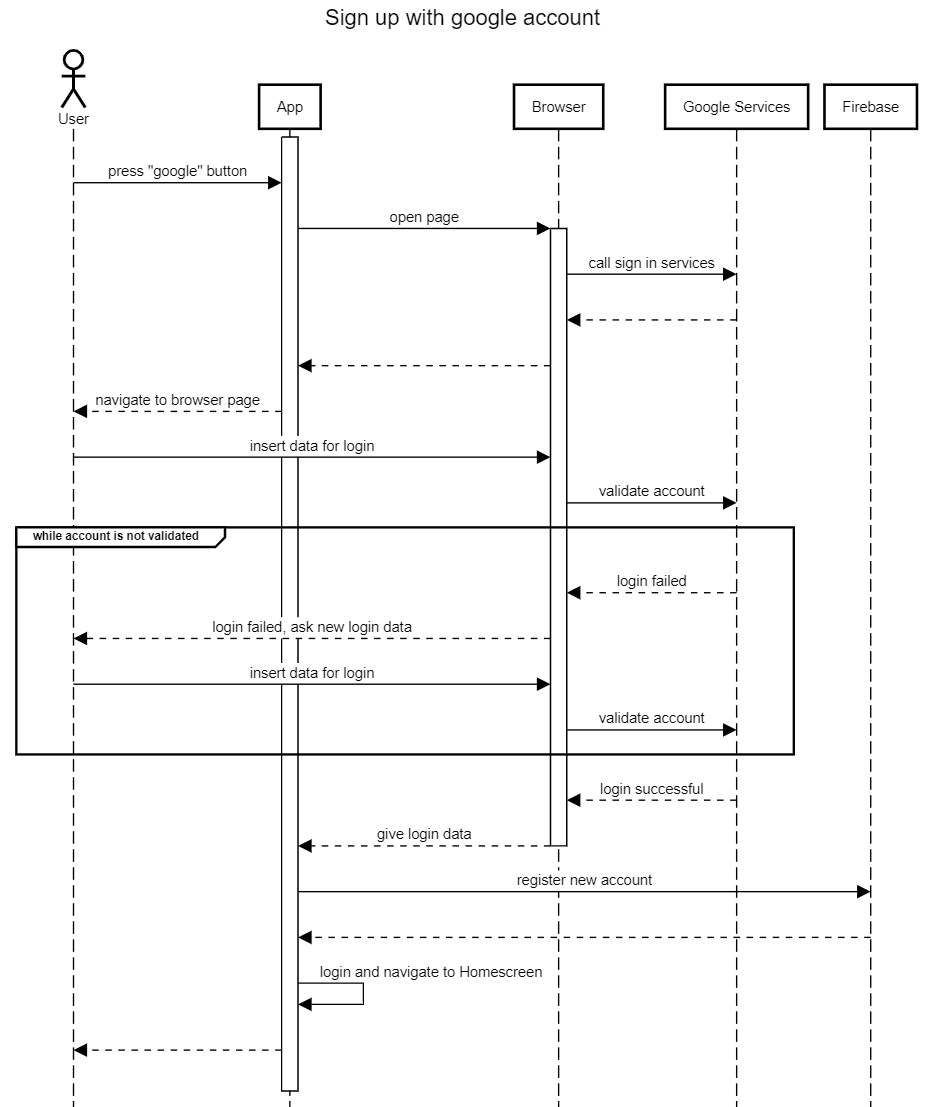
\includegraphics[scale=0.30]{resources/SignUpGoogle.png}
	\newpage
	\subsubsection{Add a plant}
	The flow to add a new plant is the longest one in \textit{Plants}. It requires a navigation through four different screens in order to add all the required data. In particular, the user has the possibility to use geolocalization or to add manually the address of the location of the plant. In this diagram the "update of the View" responses are not included to simplify the diagram.
	\newline
	\newline
	\newline
	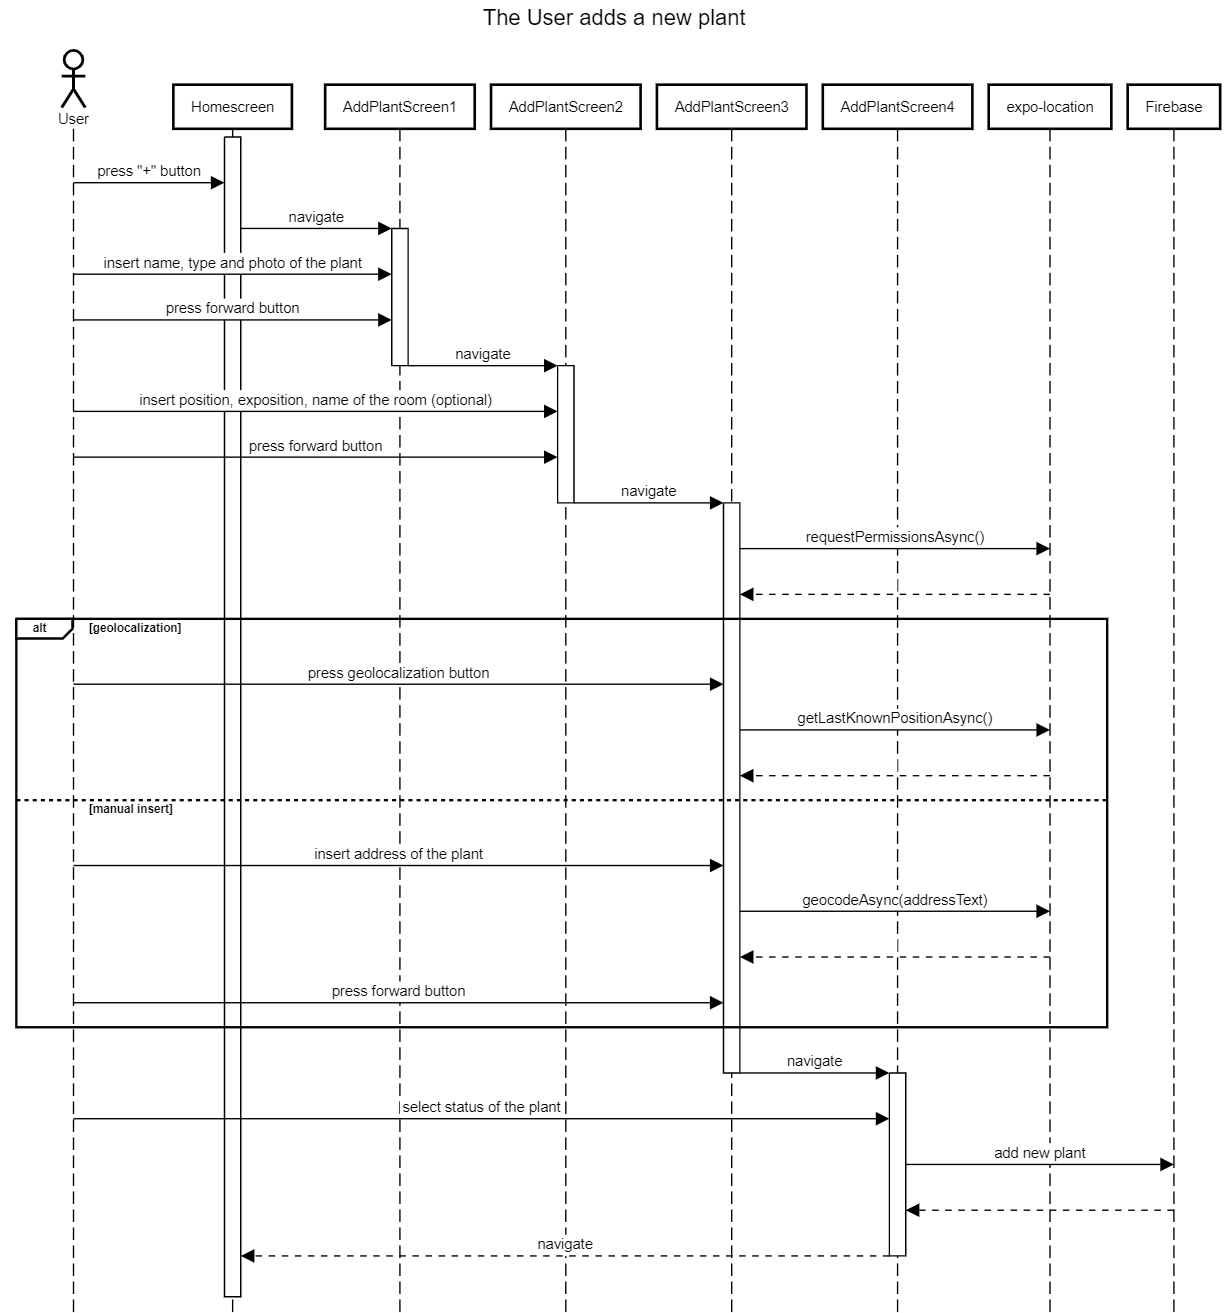
\includegraphics[scale=0.30]{resources/addPlant.png}
	\newpage
	\subsubsection{Watering event}
	The events are a core part of \textit{Plants}, since they influence the next time of watering of each plant. When an event happens, the app notifies Firebase and update its on state.
	"Good Plant" and "Bad Plant" have a similar user flow. The difference are the icon pressed, how the update of the state is done and the type of message sent to Firebase.
	\newline
	\newline
	\newline
	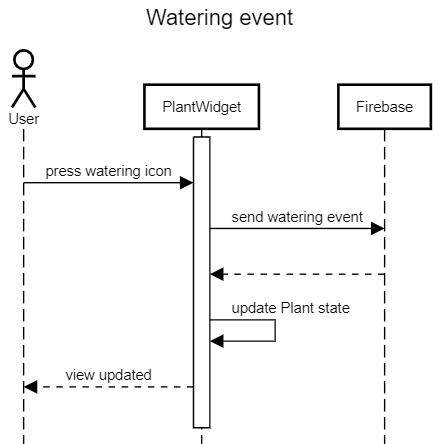
\includegraphics[scale=0.40]{resources/WateringEvent.png}
	\newpage
	\subsubsection{Delete a Plant}
	The deletion of a plant requires to send a message to the Firebase server, in order to delete the data of the plant. When the plant is deleted, the app navigates to the Homescreen.
	\newline
	\newline
	\newline
	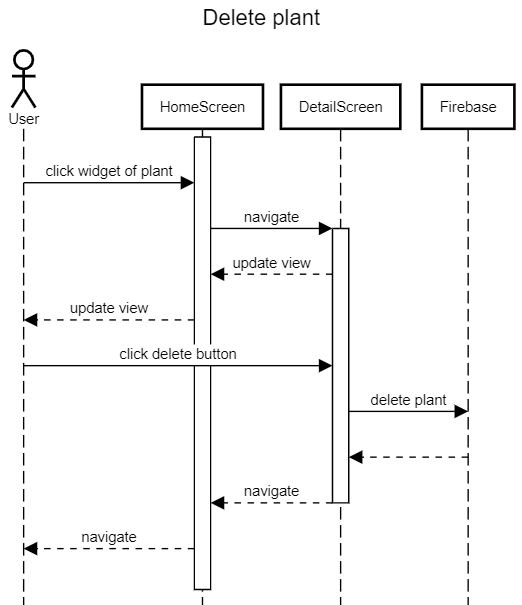
\includegraphics[scale=0.40]{resources/DeletePlant.png}
	
	\newpage
	
	\section{User Interface Design}
	In this section the interfaces of all the screens of the application are showed.
	\newline
    
    \begin{figure}[h]
     \centering
     \begin{minipage}[h]{0.4\textwidth}
         \centering
         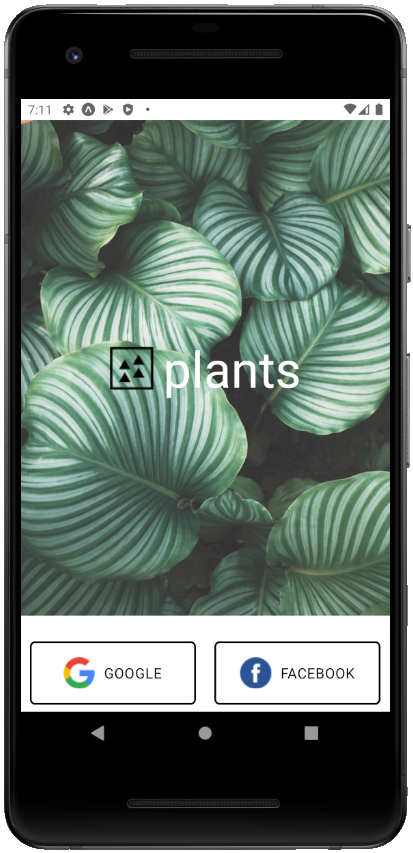
\includegraphics[width=\textwidth]{resources/screens/login.PNG}
         \caption{Login}
         \label{fig:screen1}
     \end{minipage}%
     \hfill
     \begin{minipage}[h]{0.4\textwidth}
         \centering
         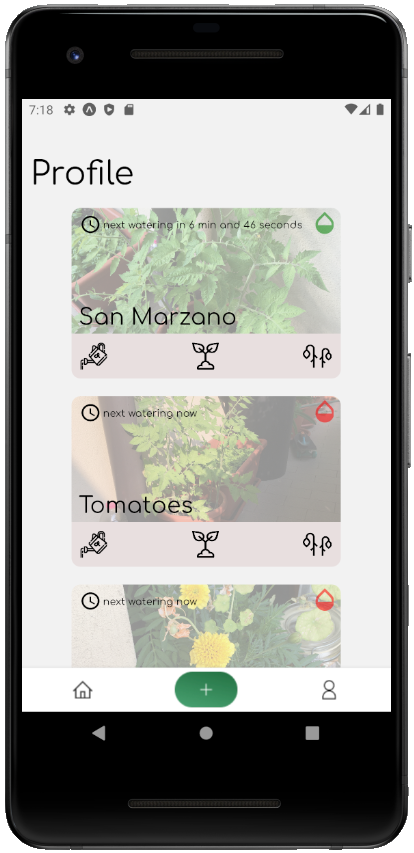
\includegraphics[width=\textwidth]{resources/screens/Homescreen.PNG}
         \caption{Homescreen}
         \label{fig:screen2}
     \end{minipage}
    \end{figure}
    
    \clearpage
    \begin{figure}[h]
     \centering
     \begin{minipage}[h]{0.4\textwidth}
         \centering
         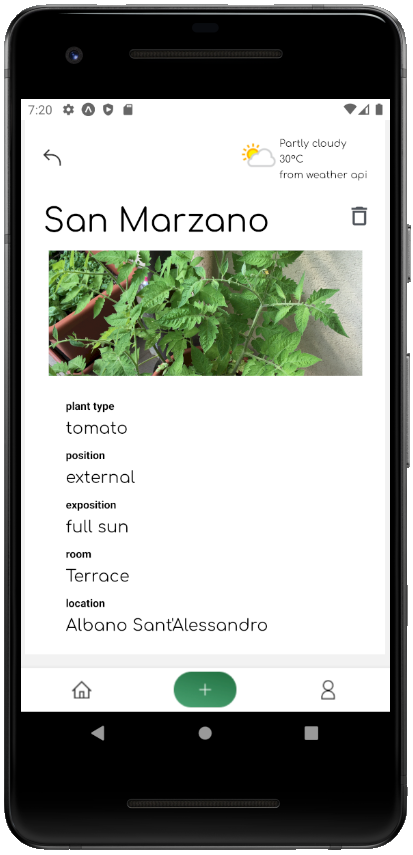
\includegraphics[width=\textwidth]{resources/screens/Details1.PNG}
         \caption{Detail of a plant}
     \end{minipage}%
     \hfill
     \begin{minipage}[h]{0.4\textwidth}
         \centering
         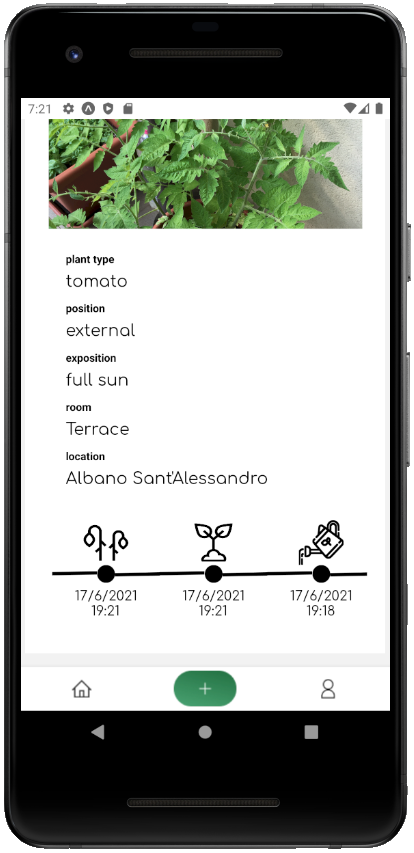
\includegraphics[width=\textwidth]{resources/screens/Details_events_2.PNG}
         \caption{Events}
     \end{minipage}
    \end{figure}
    
    \clearpage
    \begin{figure}[h]
     \centering
     \begin{minipage}[h]{0.4\textwidth}
         \centering
         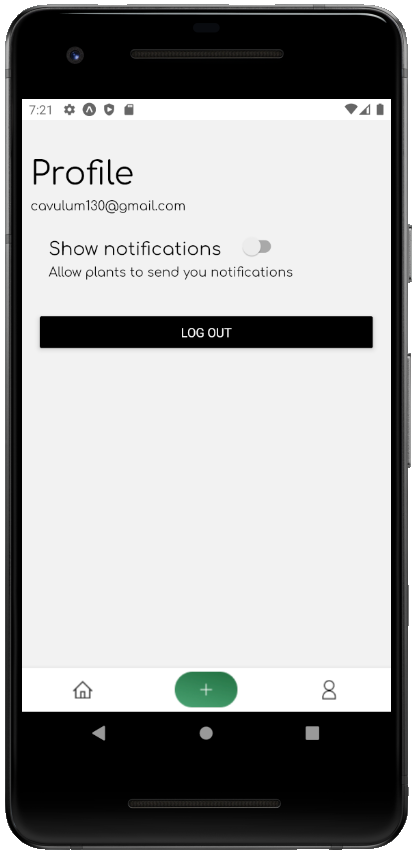
\includegraphics[width=\textwidth]{resources/screens/Profile.PNG}
         \caption{Profile}
     \end{minipage}%
    \end{figure}
    
    \clearpage
    \begin{figure}[h]
     \centering
     \begin{minipage}[h]{0.4\textwidth}
         \centering
         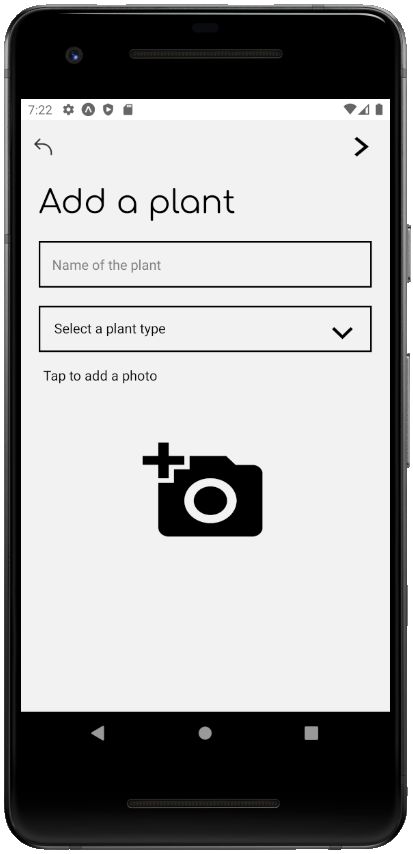
\includegraphics[width=\textwidth]{resources/screens/AddPlant1.PNG}
         \caption{Add plant 1}
     \end{minipage}%
     \hfill
     \begin{minipage}[h]{0.4\textwidth}
         \centering
         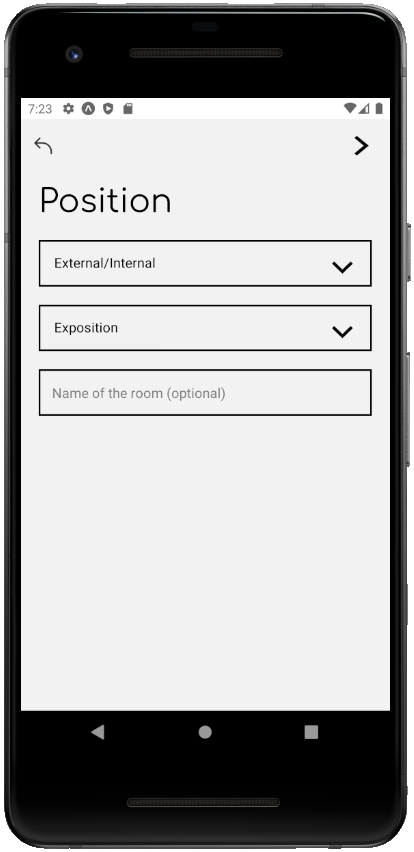
\includegraphics[width=\textwidth]{resources/screens/AddPlant2.PNG}
         \caption{Add plant 2}
     \end{minipage}
    \end{figure}
    
    \clearpage
    \begin{figure}[h]
     \centering
     \begin{minipage}[h]{0.4\textwidth}
         \centering
         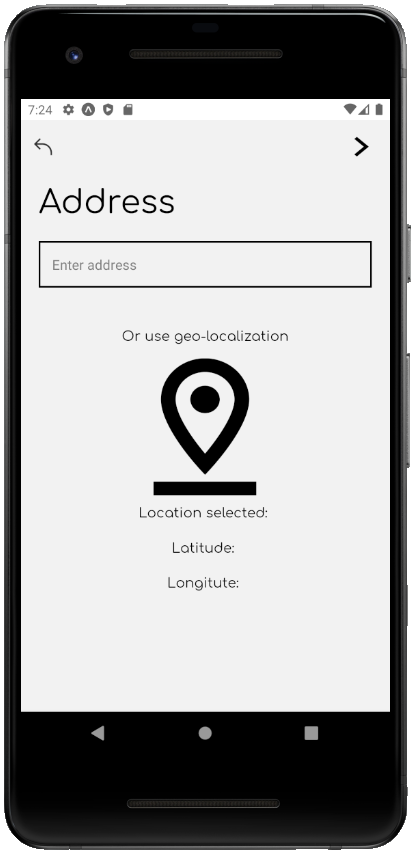
\includegraphics[width=\textwidth]{resources/screens/AddPlant3.PNG}
         \caption{Add plant 3}
     \end{minipage}%
     \hfill
     \begin{minipage}[h]{0.4\textwidth}
         \centering
         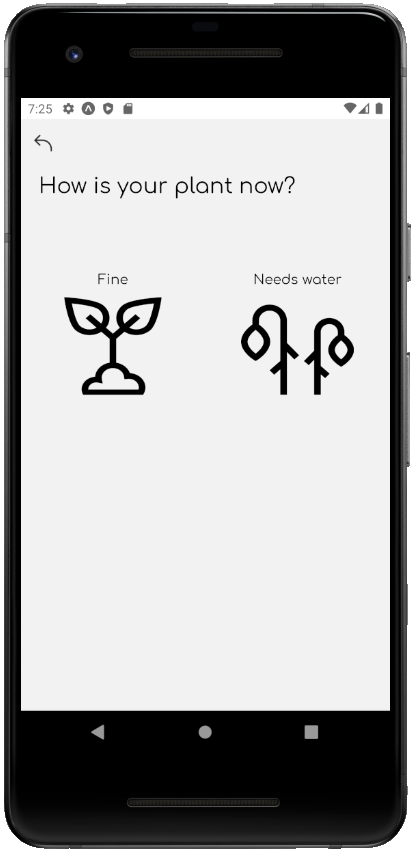
\includegraphics[width=\textwidth]{resources/screens/AddPlant4.PNG}
         \caption{Add plant 4}
     \end{minipage}
    \end{figure}
    \clearpage
	\section{Software System Attributes}
	\subsection{Reliability and Availability}
	The app requires an internet connection in order to communicate to the Firebase server. Moreover, a working camera of the smartphone is needed to add new plants. The notification system is handled by Firebase. As a consequence, an internet connection is needed to receive notifications, even if the app is not open on the smartphone. 
	\subsection{Security}
	All the data of the user is saved on Firebase, and the communication between the application the the Firebase server use the HTTPS protocol. Firebase is a a service that follows the EU General Data Protection Regulation (GDPR) and all Firebase services (aside from App Distribution and Firebase App Indexing) have successfully completed the ISO 27001 and SOC 1, SOC 2, and SOC 3 evaluation process. 
	
	Firebase also takes care of the encryption of the data, both the user login data and the plants data.
	\subsection{Maintainability}
	Using the React Native framework, the application can be easily upgraded, since the framework follows the updates of the new versions of Android and iOS.The code of the application is written following the principles of React Native programming with classes. 
	\subsection{Portability}
	The React Native framework permits to application to be run on Android and iOS devices. In particular, \textit{Plants} is meant to be used on smartphones, since its objective is to send notification to the user when plants need water. As a consequence, the app is developed to run on Android and iOS smartphones.
	\newpage
    
    \section{Testing}
    To test our result we decided to start with a black/gray box approach. This is to test as close as possible to what the user sees. In particular we scouted the testing landscape for React Native Expo and we landed short. There few major testing libraries designed specifically for this framework. \\
    We decided to test a few good candidates for mobile apps such as Appium and Detox both of whom are quite popular online.
    \subsection{Appium}
    While trying Appium we found that the architecture is quite interesting, it works like Selenium so a headless WebDriver that performs automated actions programmed by the developer. \\
    In our case we were quite attracted by the fact that tests could be written in any language of choice. \\
    While setting up we found that Appium requires an emulator, this puts us in the condition to package the app so adding another layer of complexity and in our opinion a contradiction compared to React Native Expo promises of simplicity. \\
    We decided to discard this option.
    \subsection{Detox}
    While scouting the various testing paradigms Detox came up, it is quite similar to Appium yet easier. In particular it runs natively on React Native so no WebDriver is used. While this is interesting it does not solve our emulator requirement. \\
    We decided to also discard this option.
    \subsection{Unit tests}
    We then decided to switch from black/gray box testing to white box testing. This choice came because we were looking to perform tests without setting up complex environments.
    \subsubsection{Jest}
    In particular we decided to use Jest. This tool is used to execute unit tests in the Javascript word. It is also suggested by the official React Native Expo guide so we think its a good choice.\\
    We wrote 8 unit tests to be performed on basic components and elements of the app. They are quite simple tests designed to only check that the component rendered is what we want.
    \begin{figure}[H]
    	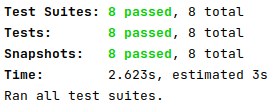
\includegraphics[scale=0.6]{resources/unittest.png}
    \end{figure}
    The tests are quite fast to run and that don't test advanced functionalities such as API calls and complex screens but they are an effective way to check for basic mistakes while developing other functionalities (regression testing).
    \subsection{Test Cases}
    To better complete the testing procedures we decided to perform also some manual test cases. This is designed to be executed by a person.
    \subsubsection{Sign In}
    The objective of this test is to check the login procedure through Google or Facebook
    \begin{center}
    	\begin{tabular}{ |c|c| } 
    		\hline
    		Initial condition & App opened\\
    		 & Google or Facebook account available on the device\\
    		\hline
    		Steps & Tap on Google or Facebook\\
    		 & Confirmation on Google or Facebook screen of identity sharing\\
    		\hline
    		Expected result & The app should navigate to the homepage\\
    		\hline
    		Passed & yes\\
    		\hline
    	\end{tabular}
    \end{center}
	\subsubsection{Add a plant}
	The objective of this test is to check the plant addition procedure
	\begin{center}
		\begin{tabular}{ |c|c| } 
			\hline
			Initial condition & App open on the homepage screen\\
			\hline
			Steps & Tap on plus sign on the bottom of the screen\\
			& Insertion of the plant name, selection of the type and taking a picture of the plant\\
			& Insertion of the Position, Exposition and optionally of the room\\
			& Insertion of the address or geolocation\\
			& Tap on the status of the plant right now\\
			\hline
			Expected result & The app should go back to the homepage and the newly added plant should be visible\\
			\hline
			Passed & yes\\
			\hline
		\end{tabular}
	\end{center}
	\subsubsection{Visualization of a plant}
	The objective of this test is to check the plant visualization features
	\begin{center}
		\begin{tabular}{ |c|c| } 
			\hline
			Initial condition & App open on the homepage screen with at least a plant available\\
			\hline
			Steps & Tap on a plant card\\
			\hline
			Expected result & The app should navigate to a screen with detailed information\\
			& about the plant, weather updates and plant history\\
			\hline
			Passed & yes\\
			\hline
		\end{tabular}
	\end{center}
	\subsubsection{Deletion of a plant}
	The objective of this test is to check the plant deletion feature
	\begin{center}
		\begin{tabular}{ |c|c| } 
			\hline
			Initial condition & App open on the plant detail screen\\
			\hline
			Steps & Tap on the bin icon in the top right of the screen\\
			\hline
			Expected result & The app should navigate to the homepage and\\
			& the plant deleted should not be visible anymore\\
			\hline
			Passed & yes\\
			\hline
		\end{tabular}
	\end{center}
	\subsubsection{Publication of a plant status}
	The objective of this test is to check the plant statuses and the insertion from the user
	\begin{center}
		\begin{tabular}{ |c|c| } 
			\hline
			Initial condition & App open on the homepage with at least one plant available\\
			\hline
			Steps & Tap on the watering icon of the plant or on the healthy icon or on the dry icon\\
			\hline
			Expected result & The app should restart the next watering timer in case of watering,\\ & increase the timespan in case of healthy and decrease it in case of dry status.\\
			& The reported status should also be available in the plant detail screen history\\
			\hline
			Passed & yes\\
			\hline
		\end{tabular}
	\end{center}
	
\end{document}
